% \textbf{Plant Identification}
% Various transfer functions of the system can be identified using the model.
% The most important one for control is \(G\) which is the transfer function from a force applied by the NASS to the measurement of the sample displacement. This represent the transfer function from \(F\) to \(d\) on Figure~\ref{fig:system_control}.

% \begin{minipage}{0.60\linewidth}
%   \begin{tikzfigure}[Transfer function from a force applied by the NASS to the sample displacement]
%   \label{fig:G_x_mass}
%   \centering
%   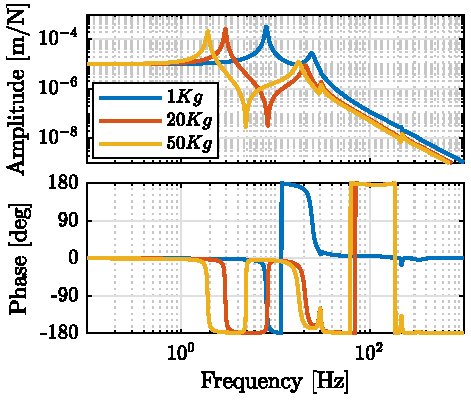
\includegraphics[height=12cm]{./figs/G_x_mass.pdf}


%   \end{tikzfigure}
% \end{minipage}\hfill
% \begin{minipage}{0.38\linewidth}
%   \begin{tikzfigure}[General control configuration]
%   \label{fig:general_conf_K}
%   \centering
%   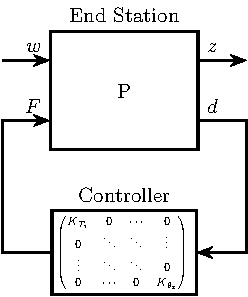
\includegraphics[height=12cm]{./figs/general_conf_K.pdf}


%   \end{tikzfigure}
% \end{minipage}\\


% As the measurement and the force applied by the NASS are in 6DoF, \(G\) is a 6 by 6 transfer function.
% Figure~\ref{fig:G_x_mass} represents the bode diagram of the first element of \(G\) for 3 values of the sample mass.
% It shows that the sample mass has an important impact on the dynamic of the system and it confirms that we will have to be very cautious about the robustness of the controlled system.

\textbf{Control Configuration}
In order to control such a system, we choose to start with a simple centralized
feedback control as shown Figure~\ref{fig:general_conf_K}.
The controller takes the signal of the metrology system in 6DoF and generates
the forces applied by the NASS in 6DoF. It is therefore a 6 by 6 matrix.
\begin{minipage}{0.49\linewidth}
  \begin{tikzfigure}[Control configuration. \(P\) is the model of the end station, \(w\) the exogenous inputs, \(d\) the 6DoF measurement, \(F\) the 6DoF forces applied by the NASS and \(z\) the signals we want to minimize.]
  \label{fig:general_conf_K}
  \centering
  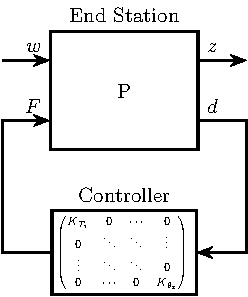
\includegraphics[height=13cm]{./figs/general_conf_K.pdf}


  \end{tikzfigure}
\end{minipage}\hfill
\begin{minipage}{0.49\linewidth}
  \begin{tikzfigure}[Positioning error of the sample during the simulation of a tomography experiment. The blue curve correspond with the ID31 without the NASS and the red curve with the NASS added. \(M=\SI{20}{\kilo\gram}\) and \(\dot{\theta_z} = \SI{30}{rpm}\).]
  \label{fig:exp_w_wo_nass_xy}
  \centering
  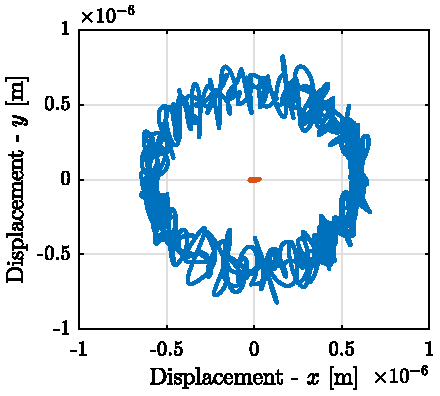
\includegraphics[height=13cm]{./figs/exp_w_wo_nass_xy.pdf}


  \end{tikzfigure}
\end{minipage}\\

\textbf{Control Synthesis}
We first choose to only have non-zero diagonal elements. Then, each diagonal
controller is tuned independently and has a lead-lag structure:
\begin{itemize}
\item An integral action is added at low frequency to have no static error
\item A lead is added near the crossover frequency to add some phase margin
\item A pole is further added in high frequency to reduce the effect of noise
\end{itemize}

\textbf{Tomography Experiment}
In order to test the performances obtained with the current controlled system, a simulation of a tomography experiment is conducted.
The rotation speed of the spindle is set to \(\dot{\theta_z} = 30rpm\), the mass of the sample is chosen to be \(M=\SI{20}{\kilo\gram}\), and ground motion is taken into account.

The result is shown Figure~\ref{fig:exp_w_wo_nass_xy}. The blue and the red curves represent the \(x-y\) motion of the sample for the positioning system respectively without the NASS and with the NASS.

The residual motion of the sample when using the NASS is less than \(\SI{50}{\nano\metre}\) in the \(xyz\) directions.

%%% Local Variables: ***
%%% mode:latex ***
%%% TeX-master: "2018 - Student Day.tex"  ***
%%% End: ***